
\section{Linear classification}

\begin{frame}
	\frametitle{Linear classification}
	
	New approach based on:
	\begin{itemize}
		\item \textbf{score function} to map raw data to class scores
		\item \textbf{loss function} to quantify the agreement between predicted and true labels
	\end{itemize}

\end{frame}

\begin{frame}
	\frametitle{Parameterised mapping from images to label scores}

	Our aim is to define the score function that maps the pixel values of an image to confidence scores for each class.

	\vskip 1cm

	Assuming that:\\
	\centering
	N images, each with dimensionality D, and K distinct classes\\
	$x_i \in R^D$ is image $i$-th with dimensions $D$ and label $y_i$,
	with $i = 1 ... N$ and $y_i \in 1 ... K$
	\vskip 1cm
	then we define a \textbf{score function}: $f: R^D \rightarrow R^K$

\end{frame}

\begin{frame}
        \frametitle{Linear classifier}

	Linear mapping:
	\centering
	$f(x_i; W, b) = W x_i + b$

	\vskip 1cm

	$W$ are called \textbf{weights} and $b$ is the \textbf{bias} vector.
	\vskip 0.5cm
	What are the dimensions of $x_i$, $W$ and $b$?\\

	\pause
	$x_i$ has size [D x 1]\\
	$W$ has size [K x D]\\
	$b$ has size [K x 1]
	

\end{frame}

\begin{frame}
	\frametitle{Linear classifier}

	\centering
	\begin{figure}
		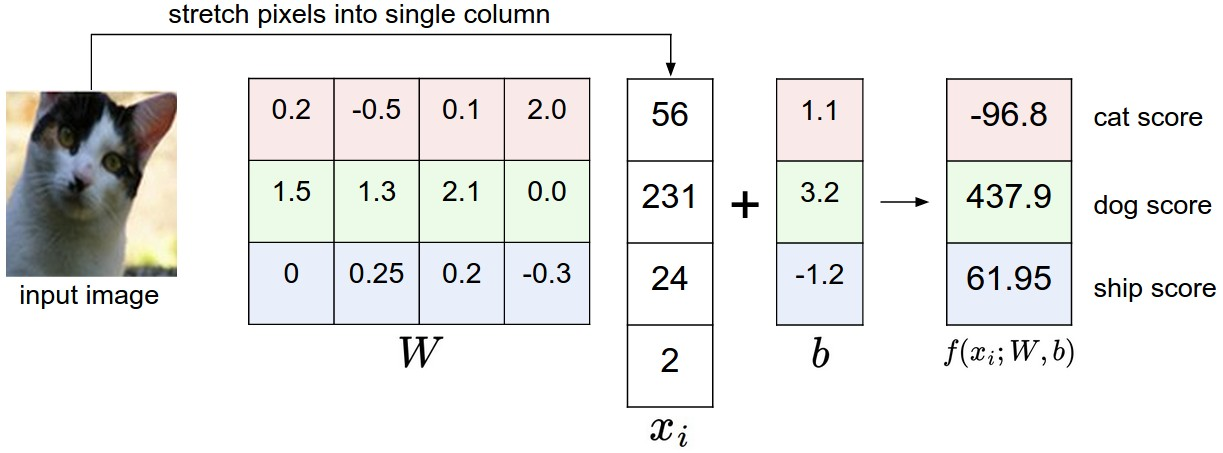
\includegraphics[width=0.9\textwidth]{Pics/imagemap.jpg}
	\end{figure}

\end{frame}


\begin{frame}
	\frametitle{Interpreting a linear classifier (i)}

	\begin{columns}
	
		\column{0.7\textwidth}
        	\begin{figure}
                	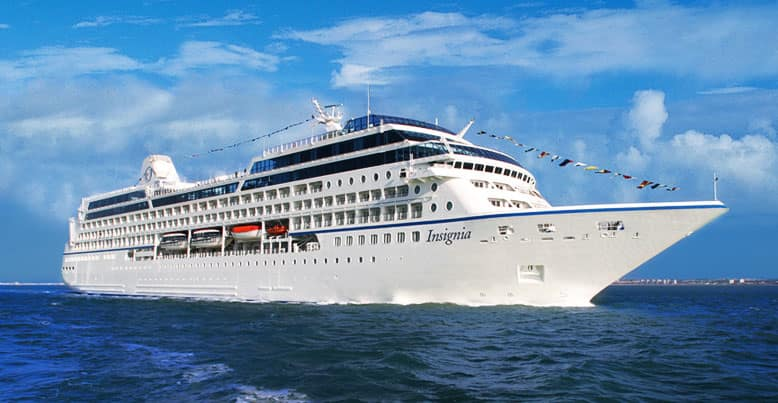
\includegraphics[width=0.8\textwidth]{Pics/ship.jpg}
        	\end{figure}

		\column{0.3\textwidth}
		\begin{figure}
                        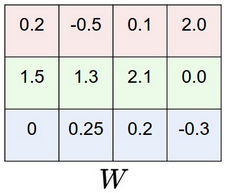
\includegraphics[width=0.8\textwidth]{Pics/W.png}
                \end{figure}
                \begin{figure}
                        
\includegraphics[width=0.6\textwidth]{Pics/like.jpg}
                \end{figure}


		
	\end{columns}

\end{frame}

\begin{frame}
        \frametitle{Interpreting a linear classifier (ii)}

        \begin{columns}
        
                \column{0.6\textwidth}
                \begin{figure}
                        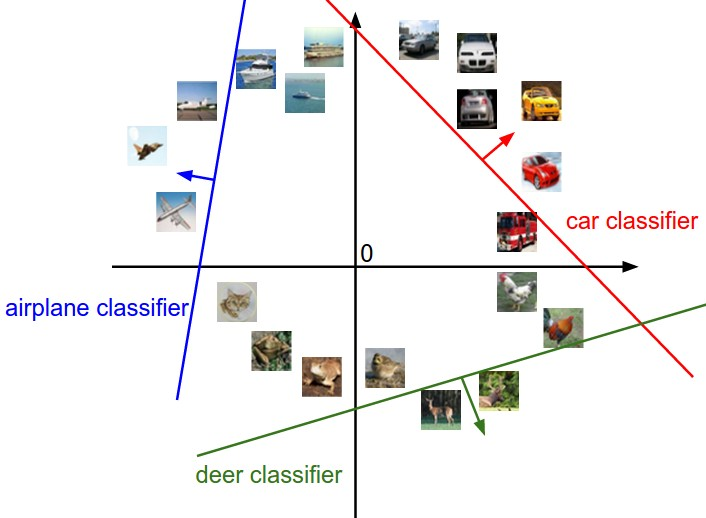
\includegraphics[width=0.9\textwidth]{Pics/pixelspace.jpeg}
                \end{figure}

                \column{0.4\textwidth}
                \begin{figure}
                        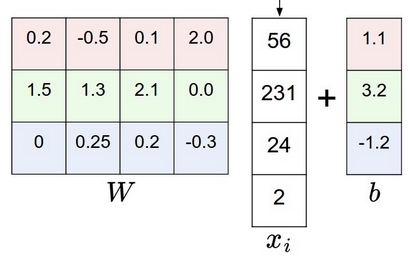
\includegraphics[width=0.9\textwidth]{Pics/Wb.png}
                \end{figure}

        \end{columns}

\end{frame}

\begin{frame}
        \frametitle{Interpreting a linear classifier (iii)}

	Template (or prototype) matching.

        \centering
        \begin{figure}
                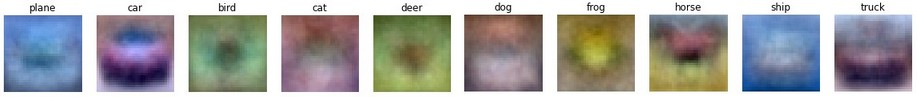
\includegraphics[width=1\textwidth]{Pics/templates.jpg}
        \end{figure}

\end{frame}

\begin{frame}
	\frametitle{Bias trick}

	Our new \textbf{score function}:\\
	$f(x_i; W) = W x_i$
	
	\begin{figure}
      		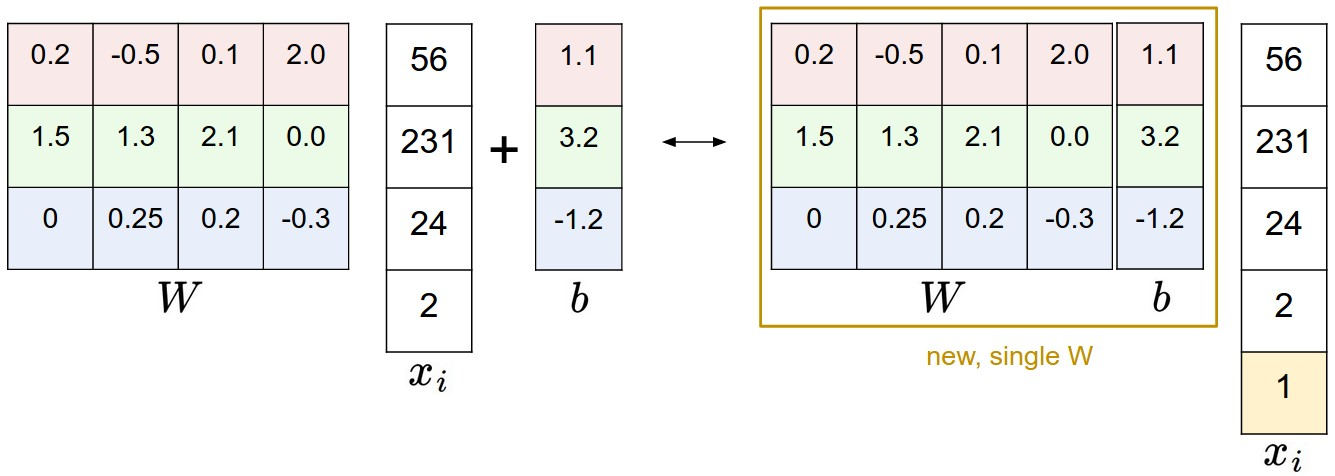
\includegraphics[width=1\textwidth]{Pics/wb.jpeg}
        \end{figure}

\end{frame}

\begin{frame}
	\frametitle{Loss function*}

	\vskip 0.5cm

	To measure our "unhappiness" with predicted outcomes.

	\begin{columns}
		\column{0.8\textwidth}
        	\begin{figure}
                	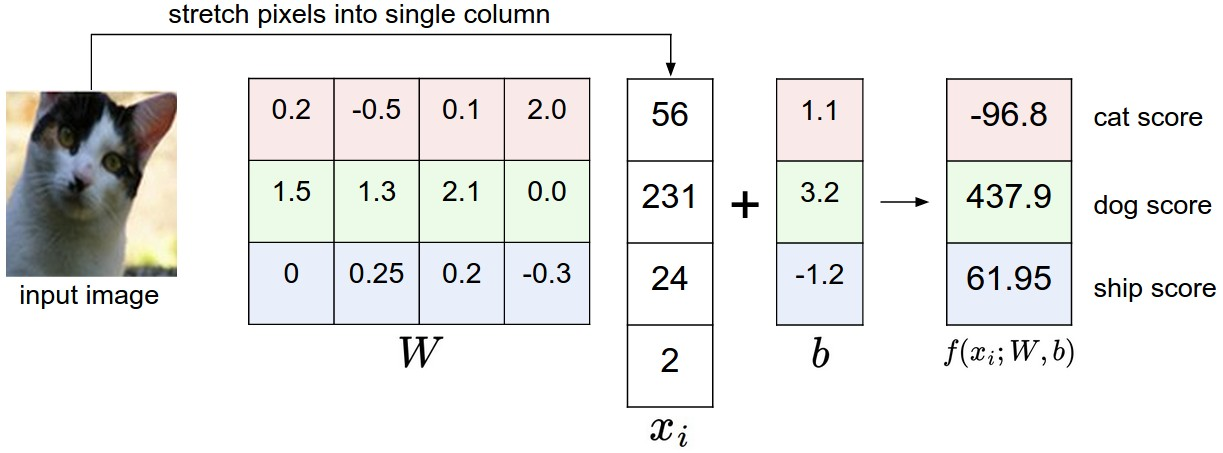
\includegraphics[width=1\textwidth]{Pics/imagemap.jpg}
        	\end{figure}
		\column{0.2\textwidth}
		\pause
                \begin{figure}
                        
\includegraphics[width=0.5\textwidth]{Pics/unhappy.png}
                \end{figure}
	\end{columns}	

	\vskip 1.5cm
	\small{* sometimes called cost function or objective}

\end{frame}

\begin{frame}
	\frametitle{Multiclass Support Vector Machine (SVM) loss}

	The SVM loss is set so that the SVM "wants" the correct class for each image to a have a higher score than the incorrect ones by some fixed margin.

	\begin{equation*}
		L_i = \sum_{j \neq y_i} max (0, s_j-s_{y_i} + \delta)
	\end{equation*}

	Example:\\
	$s=[13,-7,11]$,$y_i=0$,$\delta=10$\\
	$L_i = $ \pause $8$	

\end{frame}

\begin{frame}
        \frametitle{Hinge loss}

	$max(0,-)$ or $max(0,-)^2$

	\centering
	\begin{figure}
      		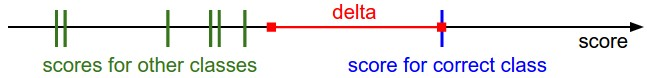
\includegraphics[width=0.9\textwidth]{Pics/margin.jpg}
     	\end{figure}
 
\end{frame}

\begin{frame}
	\frametitle{Regularisation}

	If $W$ correctly classifies each sample, then all $\lambda W$ with $\lambda>1$ will have zero loss.\\
	\vskip 0.2cm
	Which $W$ should we choose?

	\vskip 0.5cm

	\pause
	
	Our new multiclass SVM loss function is:
	\begin{equation*}
                L = \frac{1}{N} \sum_i \sum_{j \neq y_i} [max (0, f(x_i; W)_j - f(x_i; W)_{y_i} + \delta)] + \lambda \sum_k \sum_l W^2_{k,l}
        \end{equation*}
	including one data loss and one regularisation loss term $\lambda R(W)$, specifically L2 penalty.

\end{frame}

\begin{frame}
	\frametitle{Softmax classifier}

	Generalisation of the binary logistic regression classifier to multiple classes.
	\vskip 0.5cm
	Cross-entropy loss function:
	\begin{equation*}
		L_i = -\log ( \frac{ e^{f_{y_i}}} {\sum_j e^{f_j}} )
	\end{equation*}
	
\end{frame}

\begin{frame}
	\frametitle{Probabilistic interpretation of Softmax scores}

	\begin{equation*}
      		P(y_i | x_i; W) = \frac{ e^{f_{y_i}}} {\sum_j e^{f_j}}
        \end{equation*}

	Likelihood or Bayesian?

\end{frame}

\begin{frame}
	\frametitle{SVM vs. Softmax classifier}

	\centering
        \begin{figure}
                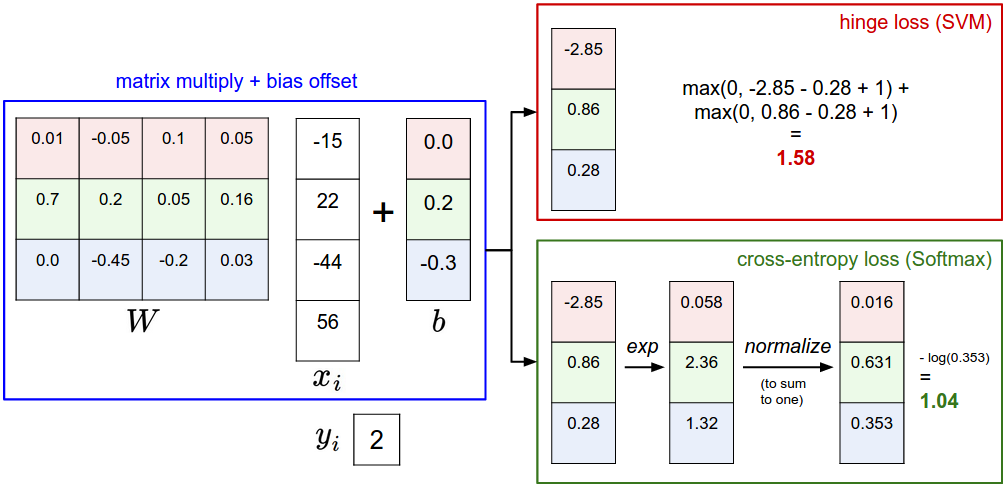
\includegraphics[width=0.9\textwidth]{Pics/svmvssoftmax.png}
        \end{figure}

\end{frame}

\begin{frame}
	\frametitle{Wrap up}

	\begin{itemize}
		\item A score function maps image pixels to class scores (using
		 a linear function that depends on W and b).
		\item Once we learning is done, we can discard the training data
		and prediction is fast.
		\item A loss function (e.g. SVM and Softmax) measures how 
		compatible a given set of parameters is with respect to the 
		ground truth labels in the training dataset. 
	\end{itemize}

	How do we determine (optimise) the parameters that give the lowest loss?

\end{frame}



